
\documentclass[10pt,a4paper]{article}
\usepackage{ifpdf}
\usepackage[utf8]{inputenc}
\usepackage[portuges]{babel}
\usepackage{csvsimple}
\usepackage{float}
\usepackage{graphicx}
\usepackage{enumerate}
\usepackage{url}
\usepackage[top=2cm,left=2cm,right=2cm,bottom=2cm]{geometry}
\title{Análise de métodos de seleção para algoritmos genéticos}
\author{Anderson Gonçalves Marco}
\usepackage{amsmath}
\usepackage{array}
\newcolumntype{L}[1]{>{\raggedright\let\newline\\\arraybackslash\hspace{0pt}}m{#1}}
\newcolumntype{C}[1]{>{\centering\let\newline\\\arraybackslash\hspace{0pt}}m{#1}}
\newcolumntype{R}[1]{>{\raggedleft\let\newline\\\arraybackslash\hspace{0pt}}m{#1}}
{\renewcommand{\arraystretch}{1.4}%
\setlength{\parindent}{0pt} % Default is 15pt.
\input{tabelas/treinamento.tex}
\begin{document}
\date{}
\maketitle
\section{Introdução}
Problemas de otimização são importantes em diferentes áreas da ciência como a engenharia de produção, mecânica e logística. Nestes tipos de problemas tenta-se conseguir o máximo de resultado com o mínimo de recursos. Os algoritmos genéticos são extremamente importantes para  resolução destes problemas, eles são métodos baseados na teoria de evolução de Charles Darwin. A sua principal característica é a habilidade para resolução de diversos problemas de otimização, sem que para isto seja necessário grandes esforços para a modelagem dos problemas.\\ \\
Os algoritmos genéticos, apesar da sua versatilidade, possuem ainda várias lacunas em sua teoria. Entre as lacunas podem ser destacadas as taxas mutação dos genes dos algoritmos e os métodos de seleção deles.\\ \\
Este artigo faz uma comparação entre os métodos de seleção por roleta e torneio, medindo a taxa de eficiência de ambos. Para esta análise foi criado um cenário de otimização por algoritmos genéticos, neste cenário foi realizado a maximização da pontuação do popular jogo de celular e computador Angry Birds. \\ \\
O ambiente do jogo Angry Birds é acessível neste trabalho através do framework AI Birds \cite{aiBirds}, sendo assim possível criar agentes para o mesmo. Podendo então ser capaz de realizar o cenário proposto, a partir deste framework. \\ \\ 
Também foi realizada comparação direta entre a pontuação alcançada pelos agentes criados por ambos os métodos de seleção citados e com o agente ``burro'' que o próprio framework do AI Birds disponibiliza.

%http://www.carlosmartins.com.br/_bizplan/bizplan05.htm
\section{Algoritmos genéticos}
Algoritmos genéticos são uma técnica da inteligência artificial para resolução de problemas. Eles foram primeiro descritos por \cite{primeiroAUsarAG} e tem como  base a teoria da evolução criada por Charles Darwin. Esta teoria diz que indivíduos mais adaptados tem mais chances de se reproduzir e assim passar suas características adiante. \\ \\
Apesar de Charles Darwin ter proposto a teoria evolução humanos já fazem seleção artificial sobre raças de animais há milhares de anos, os adaptando para o seu próprio propósito. Como exemplo da seleção artificial feita pelos humanos pode-se destacar os cachorros, que evoluíram a partir de lobos selvagens, criadores de cachorros selecionaram os lobos mais dóceis para a procriação criando assim os cachorros.\\ 
\begin{figure}[H]
  \center
  \includegraphics[scale=0.6]{imgs/cachorroELobo.jpg}            
  \caption{Um cachorro é um lobo juntos. Os cachorros são apenas lobos com genes que os deixam mais dóceis.}
  \label{fig:MostrandoOCruzamentoPorCorte}
\end{figure} 

Os algoritmos genéticos usam uma abordagem semelhante aos criadores de animais só que aplicados à vetores de dados, estes vetores são chamados de cromossomos. Cromossomos tem genes, que são os elementos do vetor, este podem ser binários, inteiros ou números reais. A Figura \ref{fig:ExemploDeVetores} ilustra estes três tipos.\\ \\
\begin{figure}[H]
  \center
  \fbox{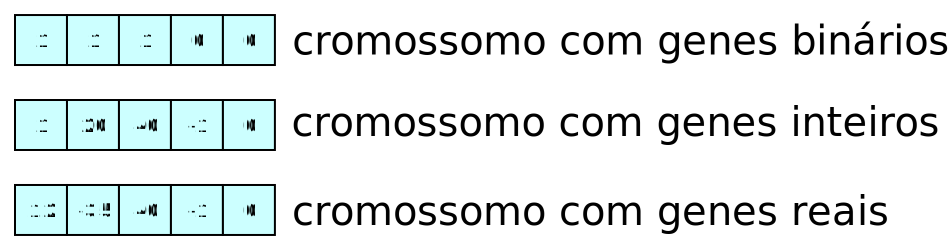
\includegraphics[scale=0.6]{imgs/tiposDeCromossomo.pdf}}            
  \caption{Os vários tipos de genes que os cromossomos podem ter.}
  \label{fig:ExemploDeVetores}
\end{figure} 

A decisão sobre quais cromossomos são melhores para transmitir seus dados para as gerações futuras, o cruzamento, pertence a função a ser otimizada, chamada de função objetivo. A função objetivo apenas da uma pontuação para um cromossomo que diz o quão bom ele é para a função, quem decide se o cromossomo vai ou não passar suas característica é o método de seleção. Existem dois principais métodos de seleção. Um dos métodos é o da roleta, descrito em \cite{UFRGS-Apostila-GA} e \cite{Livro-De-IA}, e o do torneio, descrito em   \cite{Livro-De-IA} .\\ \\
 Na seleção por roleta existem um vetor $\vec{p}$ que guarda a pontuação que cada cromossomo da geração atual recebe da função objetivo, também existe um grupo de vetores  $^i\vec{c}$ que guardam os cromossomos da geração atual. A possibilidade  $^i\vec{c}$ ser escolhido em cada cruzamento é de $\left [100 \left ( \frac{p_{i}}{\sum \limits_{j=i}^{n} p_{j}}\right ) \right ]\%$, com $n$ sendo igual ao número de elementos de $\vec{p}$. \\ \\
A seleção por torneio possui várias variantes, a utilizada neste trabalho consiste em selecionar aleatoriamente quatro cromossomos da população, chamados de $\gamma_{1},\gamma_{2},\gamma_{3}$ e $\gamma_{4}$ seleciona-se então entre $\gamma_{1}$ e $\gamma_{2}$ aquele que tem a maior pontuação, este cromossomo é chamado de $\gamma_{5}$, depois seleciona-se  entre $\gamma_{3}$ e $\gamma_{4}$ aquele que tem a maior pontuação, este cromossomo é chamado de $\gamma_{6}$. O cruzamento então é realizado entre $\gamma_{5}$ e $\gamma_{6}$. \\ \\
Após a escolha para os vetores existe um cruzamento entre eles. Neste cruzamento dois ou mais cromossomos, dos escolhidos, unem-se para criar novos cromossomos. O número de cromossomos criados por um cruzamento geralmente é igual a quantidade de cromossomos que se juntaram para o cruzamento. São duas principais maneiras  para se fazer o cruzamento, a uniforme e a por corte. \\ \\
No cruzamento por corte genes de regiões preestabelecidas dos cromossomos pais, geração atual, vão para os cromossomos filhos, geração seguinte. A Figura \ref{fig:MostrandoOCruzamentoPorCorte} mostra o cruzamento por corte. \\ 
\begin{figure}[H]
  \center
  \fbox{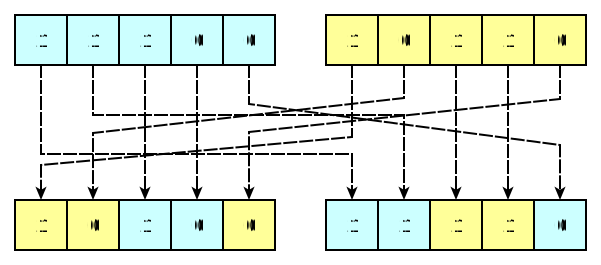
\includegraphics[scale=0.6]{imgs/diagramaCorte.pdf}}            
  \caption{Cruzamento por corte entre dois cromossomos gerando dois novos Cromossomos. Neste cruzamento existe dois pontos de corte.}
  \label{fig:MostrandoOCruzamentoPorCorte}
\end{figure} 

No cruzamento uniforme cada vez que um grupo de cromossomos pai se unem para formar filhos é gerada uma mascara, esta mascara diz que genes de um determinado cromossomo pai o filho vai receber. A Figura \ref{fig:MostrandoOCruzamentoUniforme} mostra o cruzamento uniforme. \\ \\
\begin{figure}[H]
  \center
  \fbox{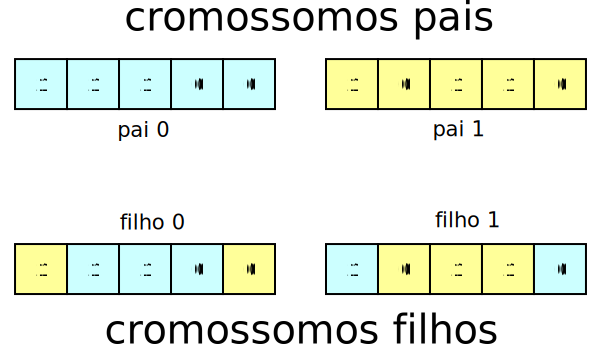
\includegraphics[scale=0.6]{imgs/diagramaMascara.pdf}}
  \caption{Cruzamento uniforme, através da mascara 10001.}
  \label{fig:MostrandoOCruzamentoUniforme}
\end{figure} \
Após o cruzamento os cromossomos criados tem uma possibilidade de ter genes alterados aleatoriamente, isto é chamado de mutação. A mutação é importante para se sair do máximo local de uma função objetivo. Porém ela não pode ser muito frequente por que uma mutação frequente faria com que os cromossomos criados fossem apenas vetores aleatórios.\\ \\
Assim os algoritmos genéticos podem ser definidos pelo fluxograma da Figura \ref{fig:DiagramaAG}. Este diagrama basicamente diz que se tem uma população inicial, geralmente gerada aleatoriamente, de cromossomos, chamada aqui de população $\alpha$.  Os cromossomos são então submetidos a uma função objetivo ela diz o quão aptos eles são. Os cromossomos são escolhidos para cruzamento com base na aptidão deles, isto gera uma nova população de cromossomos, chamada aqui de população $\beta$. Alguns genes dos cromossomos da população $\beta$ são então alterados de maneira aleatória, eles sofrem a mutação. A população $\beta$ transforma-se na população $\alpha$. Repete-se o processo novamente então por $M$ vezes.
\begin{figure}[H]
  \center
  \fbox{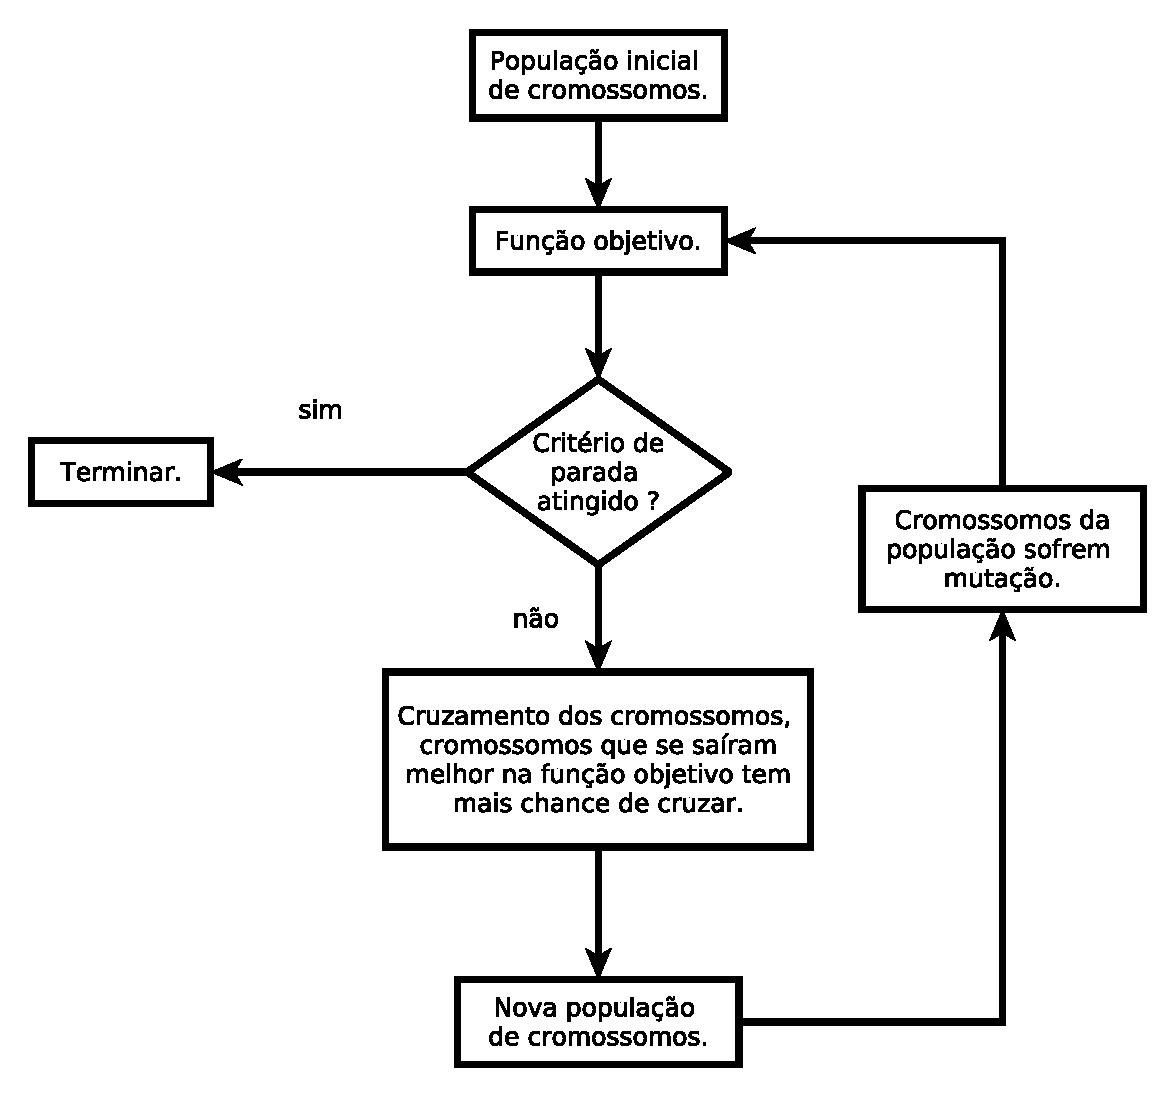
\includegraphics[scale=0.6]{imgs/diagramaAG.pdf}}            
  \caption{Fluxograma ilustrando o conceito dos algoritmos genéticos.}
  \label{fig:DiagramaAG}
\end{figure}
\subsection{Angry Birds}
\label{sec:angryBirds}
O Angry Birds é um popular jogo de dispositivos portáteis (celulares) e computadores, a Figura \ref{fig:AngryBirds} mostra um screenshot do jogo. O objetivo do jogo é jogar pássaros com um estilingue é acertar todos os porcos que estão no cenário com o menor número de pássaros possível, caso não  se acerte todos os porcos com o número de pássaros que o nível do jogo fornece perde-se a partida. A interação  e recepção de dados do ambiente do jogo para o agente é feita a partir de screenshots tiradas do jogo, o agente então usa algoritmos de visão computacional sobre estas screenshots para ter uma percepção completa, sobre a situação do jogo.   \\ \\
\begin{figure}[H]
  \center
  \includegraphics[scale=0.5]{imgs/angryBirds.png}            
  \caption{Screenshot do jogo Angry Birds.}
  \label{fig:AngryBirds}
\end{figure}
O ambiente do jogo pode ser descrito como: 
\begin{itemize}
\item Completamente observável. Pois o framework permite, através do uso de visão computacional, que o agente tenha um conhecimento sobre todas as informações pertinentes ao ambiente para que ele tome suas escolhas. Entre as informações providas pelo framework estão: Saber onde estão os inimigos, saber quais são estruturas do ambiente que são interativas e a que classe elas pertencem, saber o tipo de munição (pássaro) que está no estilingue.
\item  Não determinístico. Pois jogadas iguais produzem pontuações diferentes, o vídeo gravado em \textbf{\url{videos/naoDesterminismo.webm}} mostra isto. Isto acontece porque possivelmente a simulação física de colisão e gravidade usa métodos de monte carlo, uma vez que estes métodos de simulação são mais baratos computacionalmente. Porem não foi achado nenhum documento no site do Angry Birds dizendo isto.
\item Sequencial. Por que conforme se atira pássaros nos porcos o ambiente vai mudando.
\item Estático. Isto depende do agente, no caso da implementação realizada neste trabalho o agente espera o ambiente se estabilizar entre os arremessos dos pássaros. Por estabilizar se entende  que um novo pássaro só vai ser jogado após  o arremesso do pássaro anterior ter movido oque tinha que ser movido, os blocos e pedras do ambiente por exemplo. Isto é feito esperando-se 40 segundos entre cada arremesso de pássaro.  No entanto pode-se criar um agente que arremesse um pássaro seguido do outro, com uma pausa entre a jogadas tão pequena que enquanto um pássaro ainda está atingindo algo no ambiente (oque vai mudar o ambiente) outro já foi arremessado. 
\item Continuo.
\item Agente único. 
\end{itemize}
\section{Modelagem do Angry Birds para algoritmos genéticos}
\label{sec:modelagem}
Para a modelagem se utilizou os genes como sendo do tipo ``números reais'', para facilitar o processo de modelagem. Também se considerou que existem 3 categorias de genes, são eles:
\begin{itemize}
  \item Força, que diz com que força um pássaro é lançado do estilingue. Ele vai de  $0$ a $24$.
  \item Ângulo, que diz o ângulo em que o pássaro é arremessado. Ele vai de  $0$ a $80$.
  \item Especial, que diz o tempo, em milissegundos, para ativação do especial do pássaro a partir do momento em que o pássaro é lançado do estilingue. Ele vai de  $0$ a $2500$.
\end{itemize}

O número de genes dos cromossomos depende da quantidade de pássaros que o nível do jogo disponibiliza, pois cada pássaro deve possuir uma força de arremesso, um ângulo de arremesso e um tempo para ativação de seu especial (este gene pode ser desconsiderado para o pássaro vermelho, por ele não possuir um especial). Para o nível 20, que foi o nível em que foram realizados os testes deste trabalho, são 15 genes para cada cromossomo. Isso acontece porque este  nível possui 5 pássaros amarelos. \\ \\
Para a função objetivo desta modelagem usa-se um determinado nível do jogo Angry Birds, o 20 neste caso. Assim se submete os cromossomos, de cada geração, a arremessar um grupo de 5 pássaros (amarelos), depois dos arremessos cada cromossomo recebe do jogo uma nota por todos os seus arremessos. Como o objetivo deste trabalho é a maximização da função objetivo, ou seja obter a maior pontuação possível em um nível, os cromossomos que conseguem a maior pontuação são os mais aptos do ambiente. \\ \\
Nesta modelagem a população de cromossomos é de 40 indivíduos por geração. Os genes dos cromossomos tem probabilidade de mutação de 2.5\%. A mutação em genes da categoria força e ângulo é de até $2$ , para mais ou para menos, no valor do gene. A mutação em genes categoria especial é de até $150$, para mais ou para menos, no valor do gene. \\ \\
 Na modelagem deste trabalho, com o objetivo de tentar se preserva o máximo local, o melhor  cromossomo da geração atual sobrevive para a geração seguinte. Outra característica desta modelagem é que a cada geração um cromossomo é gerado com genes aleatórios.
\section{Resultados}
Os dois principais resultados obtidos com este trabalho foram as taxas de aprendizagem, eficiência, alcançada pelos métodos de seleção de cromossomos utilizados. Além disto foi feita uma comparação dos agentes treinados, em ambos os métodos de seleção, com o agente ``burro'' a partir do qual foram feitos os agentes deste trabalho. 
\subsection{Taxas de aprendizagem} 
Neste trabalho se considerou taxa de aprendizagem como sendo evolução da maximização da função objetivo descrita na sessão \ref{sec:modelagem}. Deste modo a taxa de aprendizagem seria a evolução da pontuação máxima obtida pela população de cromossomos conforme as gerações passam, cromossomos estes que o agente utiliza para jogar Angry Birds em um determinado nível. \\ \\
Uma outra medida, complementar a taxa de aprendizagem, seria a evolução da média da pontuação obtida pela população de cromossomos, utilizados pelo agente, conforme se avança nas gerações. \\ \\
As figuras \ref{fig:taxaAprendizagemTorneio} e \ref{fig:taxaAprendizagem2Torneio} mostram o plot da taxa de aprendizagem e media de pontuação, para quando o agente é treinado com algoritmo genético que usa o método de seleção por torneio. A figura \ref{fig:taxaAprendizagemRoleta}  mostra o plot a taxa de aprendizagem e a figura \ref{fig:taxaAprendizagem2Roleta}  mostra o plot da media de pontuação, quando o agente é treinado com algoritmo genético que usa o método de seleção por torneio. \\ \\
\begin{figure}[H]
  \center
  \fbox{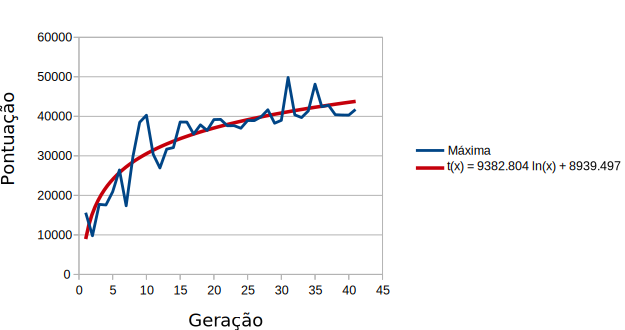
\includegraphics[scale=0.6]{imgs/plotTorneio2.pdf}}
  \caption{Taxa de aprendizagem para a algoritmo genético que usa seleção por torneio, junto a função h(x) pela qual foi ajustada.}
  \label{fig:taxaAprendizagemTorneio}
\end{figure}
\begin{figure}[H]
  \center
  \fbox{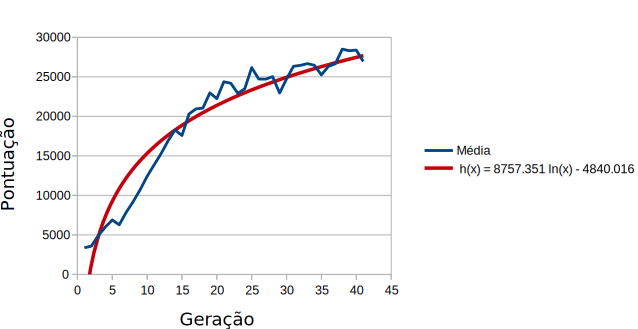
\includegraphics[scale=0.6]{imgs/plotTorneio.pdf}}            
  \caption{Media da pontuação para algoritmo genético que usa seleção por torneio, , junto a função t(x) pela qual foi ajustada.}
  \label{fig:taxaAprendizagem2Torneio}
\end{figure}
\begin{figure}[H]
  \center
  \fbox{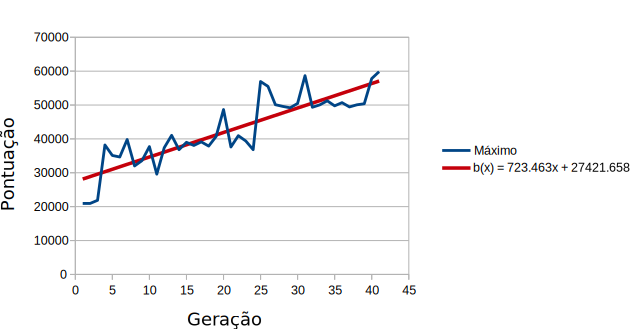
\includegraphics[scale=0.6]{imgs/plotRoleta2.pdf}}
  \caption{Taxa de aprendizagem para a algoritmo genético que usa seleção por roleta, junto a função g(x) pela qual foi ajustada.}
  \label{fig:taxaAprendizagemRoleta}
\end{figure}
\begin{figure}[H]
  \center
  \fbox{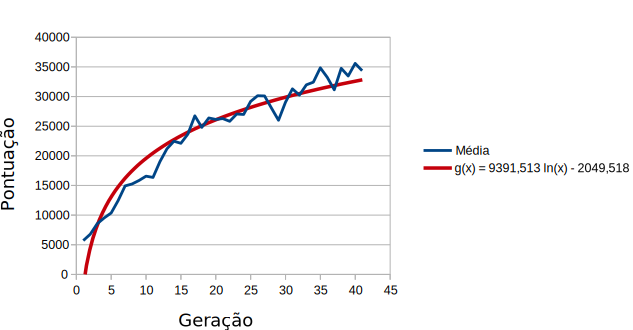
\includegraphics[scale=0.6]{imgs/plotRoleta.pdf}}
  \caption{Media da pontuação para  algoritmo genético que usa seleção por roleta, junto com a função b(x) para qual foi ajustada.}
  \label{fig:taxaAprendizagem2Roleta}
\end{figure}

Como pode-se ver o método da roleta, apresentou uma taxa de aprendizagem maior que o método do torneio. Isto pode ser visto matematicamente, derivando-se as funções $b(x)$ e $t(x)$  para as quais a taxa de aprendizagem de ambos os métodos foram ajustada. Uma vez que $b'(x)=723.463$ e $t'(x)=\frac{9382.804}{x}$ então $b'(x)>t'(x)$ pois $\lim_{x \rightarrow \infty} \frac{t'(x)}{b'(x)}<1$. O crescimento de uma função é definida pela sua derivada então $b(x)$ cresce mais rápido que $t(x)$. Mesmo que $b(x)$  fosse uma função logarítmica, o seu valor de ajuste no seria maior que o de $t(x)$\\ \\
Além disto o método da roleta também apresentou um melhor avanço na media de acertos da população de cromossomos, conforme  se passam as gerações. A demonstração matemática disto é análoga a mostrada no paragrafo anterior, basta substituir $b(x)$ por $g(x)$ e $t(x)$ por $h(x)$. \\ \\
 A Tabela  \ref{tab:tabelaDadosEvolucao} mostra os valores com os quais foram plotados os gráficos das figuras  \ref{fig:taxaAprendizagemTorneio}, \ref{fig:taxaAprendizagem2Torneio}, \ref{fig:taxaAprendizagemRoleta} e \ref{fig:taxaAprendizagem2Roleta}. \\ 
\begin{table}[h]
  \tiny
  \begin{tabular}{|l|l|l|l|l|l|l|}%
    \hline  
    \bfseries Geração & \bfseries Máximo (torneio) & \bfseries Média (torneio) & \bfseries Desvio Padrão (torneio) & \bfseries Máximo (roleta) & \bfseries Média (roleta) & \bfseries Desvio Padrão (roleta)  
                                                                                                                                                         \csvreader[head to column names]{tabelas/treinamento.csv}{}% use head of csv as column names       
                                                                                                                                                         {\\\hline \csvcoli&\csvcolii & \csvcoliii  & \csvcoliv  & \csvcolv  & \csvcolvi  & \csvcolvii  } \\ \hline
    
  \end{tabular}
  \caption{Dados estáticos referentes a pontuação das populações, de cromossomo, geradas pelo método seleção da roleta e o método do torneio.}
  \label{tab:tabelaDadosEvolucao}  
\end{table} \\
 Assim o método da roleta é melhor, do que o método  por torneio, em um ambiente de aprendizado como o descrito na seção \ref{sec:angryBirds}. 

\subsection{Comparação entre agentes treinados com o agente ``burro''}
Para esta comparação foi adotado o critério de se pegar o melhor cromossomo gerado pelo método da roleta, o melhor cromossomo gerado pelo método do torneio e comparar a pontuação que eles obtém junto com a pontuação que o agente ``burro'' obtém. \\ 
Para obter-se a pontuação a partir do agente ``burro'' se jogou o nível 20 com ele 10 vezes, com isto foi extraído uma media, desvio padrão, máximo e mínimo da pontuação dele, nas partidas de Angry Birds. \\ \\ 
Para os cromossomos utilizou-se também o critério de os agentes, criados  a partir deles, jogar 10 partidas, para poder se extrair dados estatístico a partir destas jogadas. Isto foi feito por que conforme dito na seção \ref{sec:angryBirds} o ambiente em que os agentes foram treinados possui tem um certo grau de não determinismo. \\ \\
A tabela \ref{tab:comparacaoDosAgentes} apresenta as medidas, desvios padrões, pontuações máximas e pontuações mínimas que os dois cromossomo selecionados junto com o agente ``burro'' obtiveram. \\ \\
\begin{table}[h]
  \small
  \begin{tabular}{|L{5cm}|l|l|l|l|}%
    \hline                                                                    
    \textbf{} & \textbf{Média} & \textbf{Desvio Padrão} & \textbf{Máximo} & \textbf{Mínimo} \\ \hline 
    Agente ``burro'' & 17341 & 2688.633 & 21390 & 13720 \\ \hline
    Agente criado  pelo cromossomo obtido pelo método da roleta & 31049 & 9236.183 & 47270 & 12240 \\ \hline
    Agente criado pelo cromossomo obtido pelo método do torneio & 28229 & 8720.646 & 49670  & 19950 \\ \hline
  \end{tabular}
  \caption{Dados estatísticos da pontuação que o agente ``burro'' e os agentes criados pelos cromossomos, obtidos pelos métodos roleta e torneio, conseguem no Jogo Angry Birds.}
  \label{tab:comparacaoDosAgentes}    
\end{table} \\ 

  Analisando a tabela \ref{tab:comparacaoDosAgentes} pode-se observar que o agentes criados a partir do cromossomos obtiveram uma média de pontos superior ao agente ``burro''. Em especial, o cromossomo criado a partir do método da roleta obteve uma melhor média de pontuação que o outro cromossomo. Isto confirma que o método da roleta é melhor para otimização de problemas em ambientes como o descrito na seção \ref{sec:angryBirds}.

\section{Conclusão}
Neste trabalho foi feita uma comparação entre dois métodos para seleção de cromossomo em algoritmos genéticos. Usando-se como base para comparação a maximização de pontuação, de um determinado nível, do jogo Angry Birds.  As análises mostram que o método de seleção por roleta se saiu melhor para o ambiente do jogo. \\ \\
Também foi realizada uma comparação de pontuação entre os agentes criados pelos melhores cromossomos obtidos por ambos os métodos de seleção, para algoritmos genéticos, com um agente ``burro'' disponibilizado pelo site IA-Birds. Ambos os agentes criados a partir dos cromossomos foram melhor que o agente ``burro''. Oque mostra que algoritmos genéticos é um bom método de IA para resolução de problemas como o descrito pelo ambiente do Angry Birds.
\bibliography{bibliografia}
\bibliographystyle{plain}
\end{document}
